\documentclass{article}
\usepackage[utf8]{inputenc}
\usepackage{siunitx}
\usepackage{graphics}
\usepackage[american,siunitx]{circuitikz}
\usepackage{amsmath}
\usepackage{svg} 
\usepackage{booktabs}
\usepackage{float}
\usepackage{xparse, xfp}
\usepackage{graphicx} 
\usepackage{steinmetz}
%\renewcommand{\thesubsection}{\thesection.\alph{subsection}}
\newcommand{\equal}{=}
\ExplSyntaxOn
\NewDocumentCommand{\defcon}{mm}
 {
  \cs_new:Npx #1 { \fp_eval:n { #2 } }
 }
\ExplSyntaxOff

\title{ECE2101L\\Electrical Circuit Analysis II Laboratory\\\,\\Lab 6\\Voltage and Current Phasors in Simple AC Circuits\\\,\\Report\\}
\author{Choi Tim Antony Yung\\\,\\Willis Nguyen\\Phineas Cozmiuc}
\date{9 March 2020}

\begin{document}

\clearpage\maketitle
\thispagestyle{empty}

\newpage
\setcounter{page}{1}

\section*{Objective}
The purpose of this experiment is to study the impact of frequency on impedance of circuit elements R, L and C in AC circuits and to examine the relation between voltage, current, impedance and frequency in simple RC and RL circuits.

\section{Relation of voltage, current, impedance and frequency in AC circuit with resistor and capacitor}
\begin{center}
    \begin{circuitikz}
        \draw
        (0,0) node[circ,label = 135:1]{} to[sinusoidal voltage source, l_=$v_s(t)\equal5\,cos(2\pi ft)$] (0,-2)
        (0,0) to[R=R\equal\SI{62}{\ohm}, i>^=i(t)] (4,0) node[circ, label = 45:2]{} to[C=C\equal\SI{47}{\micro\farad}] ++(0,-2) -- (0,-2)
        ;
    \end{circuitikz}
\end{center}

\subsection*{Theory}

Supposed the frequency of $v_s$ is \SI{60}{\hertz}, impedance of a capacitor is $Z_{\small{C}}=\frac{-j}{\omega C}=\frac{-j}{(2\pi60)(47\times 10^{-6})}\approx-56.44j\,\Omega=56.44\phase{-90^{\circ}}\,\Omega$ and the total impedance is $Z=Z_{\small{R}}+Z_{\small{C}}=R-\frac{j}{\omega C}\approx62-56.44j\,\Omega=83.84\phase{-42.31^{\circ}}\,\Omega$.\\

Total current can then be calculated as $I=\frac{V_s}{Z}=\frac{5\tiny{\phase{0^{\circ}}}}{83.84\tiny{\phase{-42.31^{\circ}}}}=\frac{5}{83.84}\phase{0^{\circ}-(-42.31^{\circ})}=0.05964\phase{42.31^{\circ}}\,A$

\subsection*{Result}
\begin{table}[H]
    \centering
    \resizebox{\columnwidth}{!}{%
    \begin{tabular}{rrrrrrrr}
        \toprule
        Frequency&$I$&$|Z_{\small{C}}|$&$V_2$&$I$&$|Z_{\small{C}}|$&$|I|$
        Error&$|Z_{\small{C}}|$ Error\\
        &calculated&calculated&measured&measured&measured&&\\
        \midrule
        \SI{60}{\hertz}&0.05964\phase{42.31^{\circ}}\,A&\SI{56.44}{\ohm}&3.405\phase{-46^{\circ}}\,V&0.05773\phase{43.18^{\circ}}\,A&\SI{58.98}{\ohm}&-3.20\,\%&4.51\,\%\\
        \SI{360}{\hertz}&0.07973\phase{8.627^{\circ}}\,A&\SI{9.406}{\ohm}&0.800\phase{-77^{\circ}}\,V&0.07796\phase{9.280^{\circ}}\,A&\SI{10.26}{\ohm}&-2.23\,\%&9.10\,\%\\
        \SI{600}{\hertz}&0.08031\phase{5.201^{\circ}}\,A&\SI{5.644}{\ohm}&0.500\phase{-80^{\circ}}\,V&0.07804\phase{5.840^{\circ}}\,A&\SI{6.407}{\ohm}&-2.83\,\%&13.53\,\%\\
        \SI{1800}{\hertz}&0.08061\phase{1.738^{\circ}}\,A&\SI{1.881}{\ohm}&0.170\phase{-79^{\circ}}\,V&0.07856\phase{1.960^{\circ}}\,A&\SI{2.164}{\ohm}&-2.53\,\%&15.02\,\%\\
        \SI{4800}{\hertz}&0.08064\phase{0.652^{\circ}}\,A&\SI{0.705}{\ohm}&0.070\phase{-68^{\circ}}\,V&0.07941\phase{0.750^{\circ}}\,A&\SI{0.881}{\ohm}&-1.52\,\%&24.95\,\%\\
        
        \bottomrule
    \end{tabular} }
\end{table}

\subsection*{Analysis}
The magnitude of $Z_C$ is $\frac{1}{\omega C}$. As frequency increases, angular frequency $\omega$ increases and $|Z_C|$ decreases, which is demonstrated in the following plot of $|Z_C|$ versus frequency.

The magnitude of current I is $\frac{|V_s|}{|Z|}$ and the magnitude of Z is $\sqrt{R^2+|Z_C|^2}$. As R and $V_s$ stays constant and frequency increases, angular frequency $\omega$ increases, $Z_C$ decreases, $|Z|$ decreases and $|I|$ then increases. As demonstrated in the following plot of $|I|$ versus frequency, $|I|$ increases as frequency increases.

\begin{figure}[H]
    \centering
        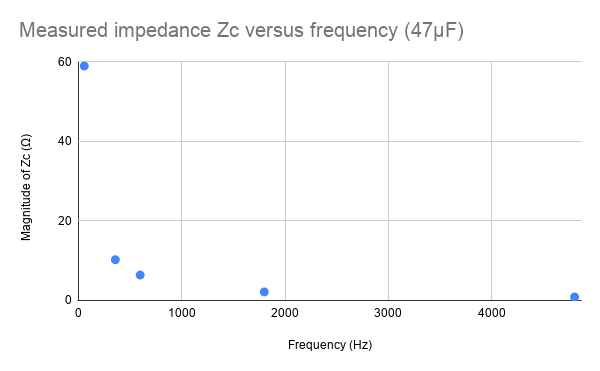
\includegraphics[scale=0.5]{ZvF_47uF.png}
\end{figure}
\begin{figure}[H]
    \centering
        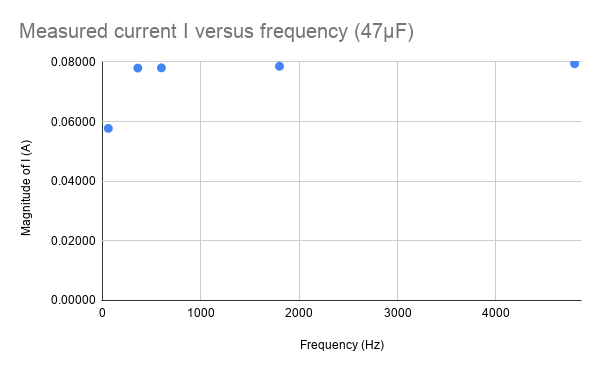
\includegraphics[scale=0.5]{IvF_47uF.png}
\end{figure}

\newpage

\section{Relation of voltage, current, impedance and frequency in AC circuit with resistor and inductor}
\begin{center}
    \begin{circuitikz}
        \draw
        (0,0) node[circ,label = 135:1]{} to[sinusoidal voltage source, l_=$v_s(t)\equal5\,cos(2\pi ft)$] (0,-2)
        (0,0) to[R=R\equal\SI{62}{\ohm}, i>^=i(t)] (4,0) node[circ, label = 45:2]{} to[L=L\equal\SI{0.8}{\henry}] ++(0,-2) -- (0,-2)
        ;
    \end{circuitikz}
\end{center}

\subsection*{Theory}

Supposed the frequency of $v_s$ is \SI{60}{\hertz}, impedance of a inductor is $Z_{\small{L}}=j\omega L=j(2\pi60)(0.8)\approx301.59j\,\Omega=301.59\phase{90^{\circ}}\,\Omega$ and the total impedance is $Z=Z_{\small{R}}+Z_{\small{L}}=R+j\omega L\approx62+301.59j\,\Omega=307.90\phase{78.38^{\circ}}\,\Omega$.\\

Total current can then be calculated as $I=\frac{V_s}{Z}=\frac{5\tiny{\phase{0^{\circ}}}}{307.90\tiny{\phase{78.38^{\circ}}}}=\frac{5}{307.90}\phase{0^{\circ}-78.38^{\circ}}=0.01624\phase{-78.38^{\circ}}\,A$

\subsection*{Result}
\begin{table}[H]
    \centering
    \resizebox{\columnwidth}{!}{%
    \begin{tabular}{rrrrrrrr}
        \toprule
        Frequency&$I$&$|Z_{\small{L}}|$&$V_2$&$I$&$|Z_{\small{C}}|$&$|I|$ Error&$|Z_{\small{L}}|$ Error\\
        &calculated&calculated&measured&measured&measured&&\\
        \midrule
        \SI{60}{\hertz}  &0.01624\phase{-78.38^{\circ}}\,A&\SI{301.59  }{\ohm}&4.705\phase{9.9^{\circ}}\,V&0.01478\phase{-62.00^{\circ}}\,A&\SI{ 318.41}{\ohm}&-9.01\,\% &5.58\,\%\\
        \SI{360}{\hertz} &0.02761\phase{-88.04^{\circ}}\,A&\SI{1809.56 }{\ohm}&5.205\phase{1.9^{\circ}}\,V&0.00287\phase{ 76.28^{\circ}}\,A&\SI{1816.62}{\ohm}&3.76\,\%  &0.39\,\%\\
        \SI{600}{\hertz} &0.01658\phase{-88.82^{\circ}}\,A&\SI{3015.93 }{\ohm}&5.235\phase{1.4^{\circ}}\,V&0.00208\phase{ 81.80^{\circ}}\,A&\SI{2511.68}{\ohm}&25.75\,\% &-16.72\,\%\\
        \SI{1800}{\hertz}&0.00553\phase{-89.61^{\circ}}\,A&\SI{9047.79 }{\ohm}&5.245\phase{1.0^{\circ}}\,V&0.00153\phase{ 75.19^{\circ}}\,A&\SI{3434.51}{\ohm}&176.35\,\%&-62.04\,\%\\
        \SI{4800}{\hertz}&0.00021\phase{-89.85^{\circ}}\,A&\SI{24127.43}{\ohm}&5.265\phase{0.5^{\circ}}\,V&0.00088\phase{ 57.03^{\circ}}\,A&\SI{5960.79}{\ohm}&326.22\,\%&-75.29\,\%\\
        
        \bottomrule
    \end{tabular} }
\end{table}

\subsection*{Analysis}
The magnitude of $Z_L$ is $\omega L$. As frequency increases, angular frequency $\omega$ increases and $|Z_L|$ increases, which is demonstrated in the following plot of $|Z_L|$ versus frequency.

The magnitude of current I is $\frac{|V_s|}{|Z|}$ and the magnitude of Z is $\sqrt{R^2+|Z_L|^2}$. As R and $V_s$ stays constant and frequency increases, angular frequency $\omega$ increases, $Z_L$ increases, $|Z|$ increases and $|I|$ then decreases. As demonstrated in the following plot of $|I|$ versus frequency, $|I|$ decreases as frequency increases.

\begin{figure}[H]
    \centering
        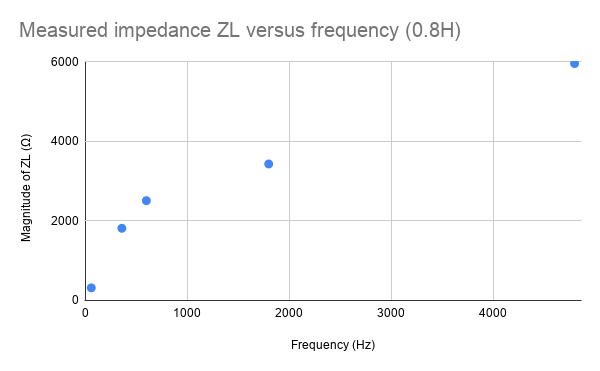
\includegraphics[scale=0.5]{ZvF_0.8H.png}
\end{figure}
\begin{figure}[H]
    \centering
        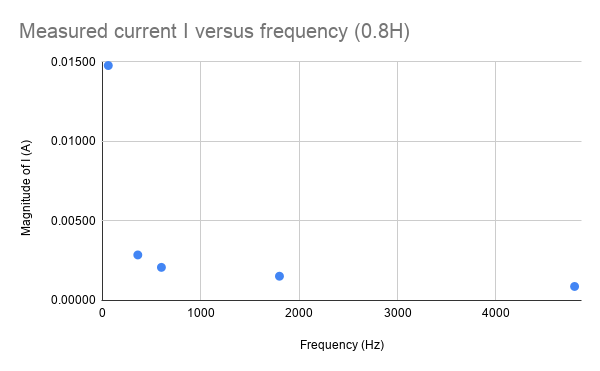
\includegraphics[scale=0.5]{IvF_0.8H.png}
\end{figure}

\end{document}